% Options for packages loaded elsewhere
\PassOptionsToPackage{unicode}{hyperref}
\PassOptionsToPackage{hyphens}{url}
%
\documentclass[
]{article}
\usepackage{lmodern}
\usepackage{amssymb,amsmath}
\usepackage{ifxetex,ifluatex}
\ifnum 0\ifxetex 1\fi\ifluatex 1\fi=0 % if pdftex
  \usepackage[T1]{fontenc}
  \usepackage[utf8]{inputenc}
  \usepackage{textcomp} % provide euro and other symbols
\else % if luatex or xetex
  \usepackage{unicode-math}
  \defaultfontfeatures{Scale=MatchLowercase}
  \defaultfontfeatures[\rmfamily]{Ligatures=TeX,Scale=1}
\fi
% Use upquote if available, for straight quotes in verbatim environments
\IfFileExists{upquote.sty}{\usepackage{upquote}}{}
\IfFileExists{microtype.sty}{% use microtype if available
  \usepackage[]{microtype}
  \UseMicrotypeSet[protrusion]{basicmath} % disable protrusion for tt fonts
}{}
\makeatletter
\@ifundefined{KOMAClassName}{% if non-KOMA class
  \IfFileExists{parskip.sty}{%
    \usepackage{parskip}
  }{% else
    \setlength{\parindent}{0pt}
    \setlength{\parskip}{6pt plus 2pt minus 1pt}}
}{% if KOMA class
  \KOMAoptions{parskip=half}}
\makeatother
\usepackage{xcolor}
\IfFileExists{xurl.sty}{\usepackage{xurl}}{} % add URL line breaks if available
\IfFileExists{bookmark.sty}{\usepackage{bookmark}}{\usepackage{hyperref}}
\hypersetup{
  pdftitle={Stats 504, F21, Assignment 1},
  hidelinks,
  pdfcreator={LaTeX via pandoc}}
\urlstyle{same} % disable monospaced font for URLs
\usepackage[margin=1in]{geometry}
\usepackage{color}
\usepackage{fancyvrb}
\newcommand{\VerbBar}{|}
\newcommand{\VERB}{\Verb[commandchars=\\\{\}]}
\DefineVerbatimEnvironment{Highlighting}{Verbatim}{commandchars=\\\{\}}
% Add ',fontsize=\small' for more characters per line
\usepackage{framed}
\definecolor{shadecolor}{RGB}{248,248,248}
\newenvironment{Shaded}{\begin{snugshade}}{\end{snugshade}}
\newcommand{\AlertTok}[1]{\textcolor[rgb]{0.94,0.16,0.16}{#1}}
\newcommand{\AnnotationTok}[1]{\textcolor[rgb]{0.56,0.35,0.01}{\textbf{\textit{#1}}}}
\newcommand{\AttributeTok}[1]{\textcolor[rgb]{0.77,0.63,0.00}{#1}}
\newcommand{\BaseNTok}[1]{\textcolor[rgb]{0.00,0.00,0.81}{#1}}
\newcommand{\BuiltInTok}[1]{#1}
\newcommand{\CharTok}[1]{\textcolor[rgb]{0.31,0.60,0.02}{#1}}
\newcommand{\CommentTok}[1]{\textcolor[rgb]{0.56,0.35,0.01}{\textit{#1}}}
\newcommand{\CommentVarTok}[1]{\textcolor[rgb]{0.56,0.35,0.01}{\textbf{\textit{#1}}}}
\newcommand{\ConstantTok}[1]{\textcolor[rgb]{0.00,0.00,0.00}{#1}}
\newcommand{\ControlFlowTok}[1]{\textcolor[rgb]{0.13,0.29,0.53}{\textbf{#1}}}
\newcommand{\DataTypeTok}[1]{\textcolor[rgb]{0.13,0.29,0.53}{#1}}
\newcommand{\DecValTok}[1]{\textcolor[rgb]{0.00,0.00,0.81}{#1}}
\newcommand{\DocumentationTok}[1]{\textcolor[rgb]{0.56,0.35,0.01}{\textbf{\textit{#1}}}}
\newcommand{\ErrorTok}[1]{\textcolor[rgb]{0.64,0.00,0.00}{\textbf{#1}}}
\newcommand{\ExtensionTok}[1]{#1}
\newcommand{\FloatTok}[1]{\textcolor[rgb]{0.00,0.00,0.81}{#1}}
\newcommand{\FunctionTok}[1]{\textcolor[rgb]{0.00,0.00,0.00}{#1}}
\newcommand{\ImportTok}[1]{#1}
\newcommand{\InformationTok}[1]{\textcolor[rgb]{0.56,0.35,0.01}{\textbf{\textit{#1}}}}
\newcommand{\KeywordTok}[1]{\textcolor[rgb]{0.13,0.29,0.53}{\textbf{#1}}}
\newcommand{\NormalTok}[1]{#1}
\newcommand{\OperatorTok}[1]{\textcolor[rgb]{0.81,0.36,0.00}{\textbf{#1}}}
\newcommand{\OtherTok}[1]{\textcolor[rgb]{0.56,0.35,0.01}{#1}}
\newcommand{\PreprocessorTok}[1]{\textcolor[rgb]{0.56,0.35,0.01}{\textit{#1}}}
\newcommand{\RegionMarkerTok}[1]{#1}
\newcommand{\SpecialCharTok}[1]{\textcolor[rgb]{0.00,0.00,0.00}{#1}}
\newcommand{\SpecialStringTok}[1]{\textcolor[rgb]{0.31,0.60,0.02}{#1}}
\newcommand{\StringTok}[1]{\textcolor[rgb]{0.31,0.60,0.02}{#1}}
\newcommand{\VariableTok}[1]{\textcolor[rgb]{0.00,0.00,0.00}{#1}}
\newcommand{\VerbatimStringTok}[1]{\textcolor[rgb]{0.31,0.60,0.02}{#1}}
\newcommand{\WarningTok}[1]{\textcolor[rgb]{0.56,0.35,0.01}{\textbf{\textit{#1}}}}
\usepackage{longtable,booktabs}
% Correct order of tables after \paragraph or \subparagraph
\usepackage{etoolbox}
\makeatletter
\patchcmd\longtable{\par}{\if@noskipsec\mbox{}\fi\par}{}{}
\makeatother
% Allow footnotes in longtable head/foot
\IfFileExists{footnotehyper.sty}{\usepackage{footnotehyper}}{\usepackage{footnote}}
\makesavenoteenv{longtable}
\usepackage{graphicx,grffile}
\makeatletter
\def\maxwidth{\ifdim\Gin@nat@width>\linewidth\linewidth\else\Gin@nat@width\fi}
\def\maxheight{\ifdim\Gin@nat@height>\textheight\textheight\else\Gin@nat@height\fi}
\makeatother
% Scale images if necessary, so that they will not overflow the page
% margins by default, and it is still possible to overwrite the defaults
% using explicit options in \includegraphics[width, height, ...]{}
\setkeys{Gin}{width=\maxwidth,height=\maxheight,keepaspectratio}
% Set default figure placement to htbp
\makeatletter
\def\fps@figure{htbp}
\makeatother
\setlength{\emergencystretch}{3em} % prevent overfull lines
\providecommand{\tightlist}{%
  \setlength{\itemsep}{0pt}\setlength{\parskip}{0pt}}
\setcounter{secnumdepth}{5}

\title{Stats 504, F21, Assignment 1}
\author{}
\date{\vspace{-2.5em}September 17, 2021}

\begin{document}
\maketitle

\hypertarget{introduction}{%
\section{Introduction}\label{introduction}}

Derogatory credit reports will exert negative effect on individual's
credit history typically for seven to ten years. It is quite crucial to
identify the factors that could potentially contribute to derogatory
reports. This analysis explains the number of credit reports in terms of
the background factors of applicants. The model shows that
\texttt{share}, \texttt{owner} and \texttt{active} have strong influence
on the derogatory reports.

\hypertarget{method}{%
\section{Method}\label{method}}

In this analysis, our target is to figure out which background factors
are associated with the number of derogatory credit reports and measure
the level of each association. In this problem, the response variable
(derogatory credit reports) is count data, as our client did, we
primarily use Poisson regression to model the count of reports with
respect to all the background factors that can potentially influence the
outcome. As our goal is to broadly understand associations between the
derogatory reports and background factors, it is reasonable to include
all the variables available in the data except \texttt{card}, because
\texttt{card} is influenced by the number of derogatory credit reports.
Our client is concerning that there are too many zeros in the report
variable, which makes the data no longer follow a true Poisson
distribution.

\begin{figure}

{\centering 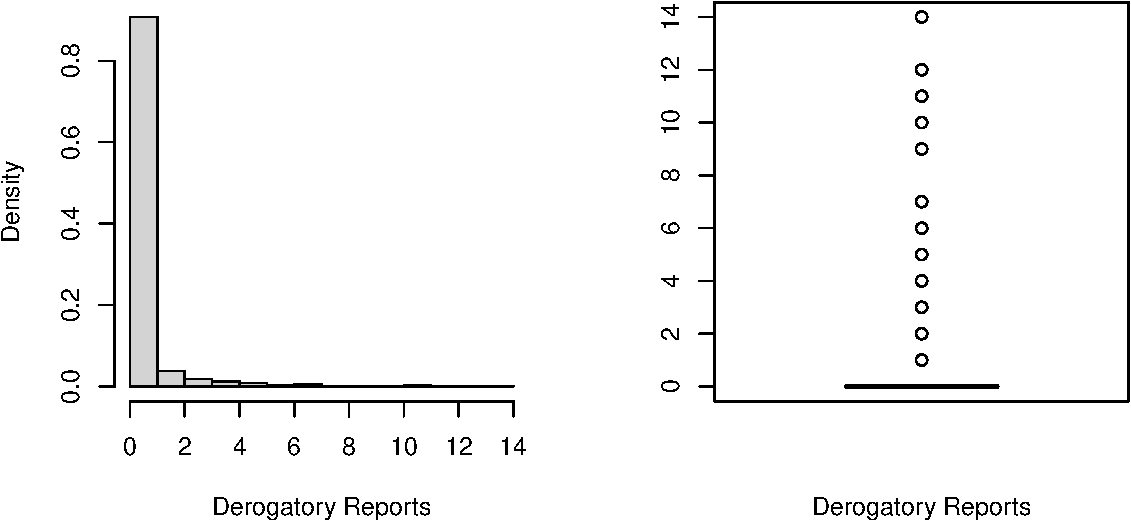
\includegraphics{stats504_hw1_files/figure-latex/unnamed-chunk-1-1} 

}

\caption{Histogram and Boxplot of Derogatory Credit Reports}\label{fig:unnamed-chunk-1}
\end{figure}

Through the above histogram, we can see that more than 80\% of the
applicants have no derogatory credit reports at all. The distribution of
derogatory reports is obviously not a Poisson distribution. Here we
consider zero-inflated models to address this problem.

We compare several different models to pursue an optimal fit for the
model shown below using likelihood-based metrics and compare them by
AIC. To ensure the easy interpretability of the model, we do not
consider variable transformation after considering model diagnostics.
Eventually we choose Zero-Inflated Negative Binomial regression model
for its lowest AIC. Detailed formula for this model can be found in the
appendix.

\hypertarget{result}{%
\section{Result}\label{result}}

The whole dataset contains 1319 observations and 12 variables. Since we
use \texttt{reports} as our outcome variable and exclude \texttt{card},
there is 10 variables left to be used as predictors. Among these
predictors \texttt{owner}, \texttt{selfemp} and \texttt{majorcards} are
binary variables with values `yes' and `no', and others predictors are
all numerical variables. Here we encode the binary variables as number
with value 1 for `yes' and 0 for `no'. There are no missing values in
this dataset, but some abnormal values. We noticed that there are 7
minor applicants with age less than 1 but high income, and all the other
observations are older than 18.

\begin{longtable}[]{@{}rrrrrrrrrrr@{}}
\toprule
\begin{minipage}[b]{0.06\columnwidth}\raggedleft
reports\strut
\end{minipage} & \begin{minipage}[b]{0.05\columnwidth}\raggedleft
age\strut
\end{minipage} & \begin{minipage}[b]{0.06\columnwidth}\raggedleft
income\strut
\end{minipage} & \begin{minipage}[b]{0.05\columnwidth}\raggedleft
share\strut
\end{minipage} & \begin{minipage}[b]{0.10\columnwidth}\raggedleft
expenditure\strut
\end{minipage} & \begin{minipage}[b]{0.05\columnwidth}\raggedleft
owner\strut
\end{minipage} & \begin{minipage}[b]{0.06\columnwidth}\raggedleft
selfemp\strut
\end{minipage} & \begin{minipage}[b]{0.09\columnwidth}\raggedleft
dependents\strut
\end{minipage} & \begin{minipage}[b]{0.06\columnwidth}\raggedleft
months\strut
\end{minipage} & \begin{minipage}[b]{0.09\columnwidth}\raggedleft
majorcards\strut
\end{minipage} & \begin{minipage}[b]{0.06\columnwidth}\raggedleft
active\strut
\end{minipage}\tabularnewline
\midrule
\endhead
\begin{minipage}[t]{0.06\columnwidth}\raggedleft
0\strut
\end{minipage} & \begin{minipage}[t]{0.05\columnwidth}\raggedleft
0.500\strut
\end{minipage} & \begin{minipage}[t]{0.06\columnwidth}\raggedleft
3.05\strut
\end{minipage} & \begin{minipage}[t]{0.05\columnwidth}\raggedleft
0.102\strut
\end{minipage} & \begin{minipage}[t]{0.10\columnwidth}\raggedleft
258.549\strut
\end{minipage} & \begin{minipage}[t]{0.05\columnwidth}\raggedleft
0\strut
\end{minipage} & \begin{minipage}[t]{0.06\columnwidth}\raggedleft
0\strut
\end{minipage} & \begin{minipage}[t]{0.09\columnwidth}\raggedleft
1\strut
\end{minipage} & \begin{minipage}[t]{0.06\columnwidth}\raggedleft
94\strut
\end{minipage} & \begin{minipage}[t]{0.09\columnwidth}\raggedleft
1\strut
\end{minipage} & \begin{minipage}[t]{0.06\columnwidth}\raggedleft
5\strut
\end{minipage}\tabularnewline
\begin{minipage}[t]{0.06\columnwidth}\raggedleft
0\strut
\end{minipage} & \begin{minipage}[t]{0.05\columnwidth}\raggedleft
0.167\strut
\end{minipage} & \begin{minipage}[t]{0.06\columnwidth}\raggedleft
3.24\strut
\end{minipage} & \begin{minipage}[t]{0.05\columnwidth}\raggedleft
0.184\strut
\end{minipage} & \begin{minipage}[t]{0.10\columnwidth}\raggedleft
497.706\strut
\end{minipage} & \begin{minipage}[t]{0.05\columnwidth}\raggedleft
1\strut
\end{minipage} & \begin{minipage}[t]{0.06\columnwidth}\raggedleft
0\strut
\end{minipage} & \begin{minipage}[t]{0.09\columnwidth}\raggedleft
3\strut
\end{minipage} & \begin{minipage}[t]{0.06\columnwidth}\raggedleft
25\strut
\end{minipage} & \begin{minipage}[t]{0.09\columnwidth}\raggedleft
1\strut
\end{minipage} & \begin{minipage}[t]{0.06\columnwidth}\raggedleft
16\strut
\end{minipage}\tabularnewline
\begin{minipage}[t]{0.06\columnwidth}\raggedleft
0\strut
\end{minipage} & \begin{minipage}[t]{0.05\columnwidth}\raggedleft
0.583\strut
\end{minipage} & \begin{minipage}[t]{0.06\columnwidth}\raggedleft
2.50\strut
\end{minipage} & \begin{minipage}[t]{0.05\columnwidth}\raggedleft
0.083\strut
\end{minipage} & \begin{minipage}[t]{0.10\columnwidth}\raggedleft
173.023\strut
\end{minipage} & \begin{minipage}[t]{0.05\columnwidth}\raggedleft
0\strut
\end{minipage} & \begin{minipage}[t]{0.06\columnwidth}\raggedleft
0\strut
\end{minipage} & \begin{minipage}[t]{0.09\columnwidth}\raggedleft
0\strut
\end{minipage} & \begin{minipage}[t]{0.06\columnwidth}\raggedleft
150\strut
\end{minipage} & \begin{minipage}[t]{0.09\columnwidth}\raggedleft
1\strut
\end{minipage} & \begin{minipage}[t]{0.06\columnwidth}\raggedleft
5\strut
\end{minipage}\tabularnewline
\begin{minipage}[t]{0.06\columnwidth}\raggedleft
0\strut
\end{minipage} & \begin{minipage}[t]{0.05\columnwidth}\raggedleft
0.750\strut
\end{minipage} & \begin{minipage}[t]{0.06\columnwidth}\raggedleft
3.00\strut
\end{minipage} & \begin{minipage}[t]{0.05\columnwidth}\raggedleft
0.000\strut
\end{minipage} & \begin{minipage}[t]{0.10\columnwidth}\raggedleft
0.000\strut
\end{minipage} & \begin{minipage}[t]{0.05\columnwidth}\raggedleft
0\strut
\end{minipage} & \begin{minipage}[t]{0.06\columnwidth}\raggedleft
0\strut
\end{minipage} & \begin{minipage}[t]{0.09\columnwidth}\raggedleft
0\strut
\end{minipage} & \begin{minipage}[t]{0.06\columnwidth}\raggedleft
18\strut
\end{minipage} & \begin{minipage}[t]{0.09\columnwidth}\raggedleft
0\strut
\end{minipage} & \begin{minipage}[t]{0.06\columnwidth}\raggedleft
2\strut
\end{minipage}\tabularnewline
\begin{minipage}[t]{0.06\columnwidth}\raggedleft
0\strut
\end{minipage} & \begin{minipage}[t]{0.05\columnwidth}\raggedleft
0.583\strut
\end{minipage} & \begin{minipage}[t]{0.06\columnwidth}\raggedleft
4.00\strut
\end{minipage} & \begin{minipage}[t]{0.05\columnwidth}\raggedleft
0.073\strut
\end{minipage} & \begin{minipage}[t]{0.10\columnwidth}\raggedleft
242.128\strut
\end{minipage} & \begin{minipage}[t]{0.05\columnwidth}\raggedleft
1\strut
\end{minipage} & \begin{minipage}[t]{0.06\columnwidth}\raggedleft
0\strut
\end{minipage} & \begin{minipage}[t]{0.09\columnwidth}\raggedleft
3\strut
\end{minipage} & \begin{minipage}[t]{0.06\columnwidth}\raggedleft
24\strut
\end{minipage} & \begin{minipage}[t]{0.09\columnwidth}\raggedleft
1\strut
\end{minipage} & \begin{minipage}[t]{0.06\columnwidth}\raggedleft
4\strut
\end{minipage}\tabularnewline
\begin{minipage}[t]{0.06\columnwidth}\raggedleft
1\strut
\end{minipage} & \begin{minipage}[t]{0.05\columnwidth}\raggedleft
0.500\strut
\end{minipage} & \begin{minipage}[t]{0.06\columnwidth}\raggedleft
3.70\strut
\end{minipage} & \begin{minipage}[t]{0.05\columnwidth}\raggedleft
0.011\strut
\end{minipage} & \begin{minipage}[t]{0.10\columnwidth}\raggedleft
32.464\strut
\end{minipage} & \begin{minipage}[t]{0.05\columnwidth}\raggedleft
0\strut
\end{minipage} & \begin{minipage}[t]{0.06\columnwidth}\raggedleft
0\strut
\end{minipage} & \begin{minipage}[t]{0.09\columnwidth}\raggedleft
0\strut
\end{minipage} & \begin{minipage}[t]{0.06\columnwidth}\raggedleft
186\strut
\end{minipage} & \begin{minipage}[t]{0.09\columnwidth}\raggedleft
0\strut
\end{minipage} & \begin{minipage}[t]{0.06\columnwidth}\raggedleft
5\strut
\end{minipage}\tabularnewline
\begin{minipage}[t]{0.06\columnwidth}\raggedleft
0\strut
\end{minipage} & \begin{minipage}[t]{0.05\columnwidth}\raggedleft
0.750\strut
\end{minipage} & \begin{minipage}[t]{0.06\columnwidth}\raggedleft
1.60\strut
\end{minipage} & \begin{minipage}[t]{0.05\columnwidth}\raggedleft
0.154\strut
\end{minipage} & \begin{minipage}[t]{0.10\columnwidth}\raggedleft
205.254\strut
\end{minipage} & \begin{minipage}[t]{0.05\columnwidth}\raggedleft
0\strut
\end{minipage} & \begin{minipage}[t]{0.06\columnwidth}\raggedleft
0\strut
\end{minipage} & \begin{minipage}[t]{0.09\columnwidth}\raggedleft
0\strut
\end{minipage} & \begin{minipage}[t]{0.06\columnwidth}\raggedleft
1\strut
\end{minipage} & \begin{minipage}[t]{0.09\columnwidth}\raggedleft
1\strut
\end{minipage} & \begin{minipage}[t]{0.06\columnwidth}\raggedleft
9\strut
\end{minipage}\tabularnewline
\bottomrule
\end{longtable}

Hence, we just directly remove these 7 observations. The following
tables shows the distribution metrics of all the variables after
processing.

\begin{longtable}[]{@{}lrrrrrr@{}}
\toprule
& Min. & 1st Qu. & Median & Mean & 3rd Qu. & Max.\tabularnewline
\midrule
\endhead
reports & 0.000 & 0.000 & 0.000 & 0.458 & 0.000 & 14.000\tabularnewline
age & 18.167 & 25.417 & 31.292 & 33.387 & 39.417 & 83.500\tabularnewline
income & 0.210 & 2.237 & 2.900 & 3.367 & 4.000 & 13.500\tabularnewline
share & 0.000 & 0.002 & 0.039 & 0.069 & 0.094 & 0.906\tabularnewline
expenditure & 0.000 & 4.583 & 101.232 & 184.970 & 248.971 &
3099.505\tabularnewline
owner & 0.000 & 0.000 & 0.000 & 0.441 & 1.000 & 1.000\tabularnewline
selfemp & 0.000 & 0.000 & 0.000 & 0.069 & 0.000 & 1.000\tabularnewline
dependents & 0.000 & 0.000 & 1.000 & 0.994 & 2.000 &
6.000\tabularnewline
months & 0.000 & 12.000 & 30.000 & 55.183 & 72.000 &
540.000\tabularnewline
majorcards & 0.000 & 1.000 & 1.000 & 0.818 & 1.000 &
1.000\tabularnewline
active & 0.000 & 2.000 & 6.000 & 6.999 & 11.000 & 46.000\tabularnewline
\bottomrule
\end{longtable}

Here we tried three models to fit the data: Poisson Regressions,
Zero-Inflated Poisson Regression and Zero-Inflated Negative Binomial
Regression. The following table shows the AIC of each model.

\begin{longtable}[]{@{}ll@{}}
\toprule
Model & AIC\tabularnewline
\midrule
\endhead
Poisson Regressions & 2514.59\tabularnewline
Zero-Inflated Poisson Regression & 2090.59\tabularnewline
Zero-Inflated Negative Binomial Regression & 1912.04\tabularnewline
\bottomrule
\end{longtable}

Through this table, we can see that zero-inflated model can significant
decrease the AIC of the model, which is definitely a better fit than the
original model. Within the zero-inflated models, negative binomial
regression model can achieve a better fit than the Poisson regression
model. Hence, the final model here we choose is Zero-Inflated Negative
Binomial Regression with AIC equals 1912.04. The model details are
presented below:

\begin{Shaded}
\begin{Highlighting}[]
\NormalTok{reportsZifNB =}\StringTok{ }\KeywordTok{zeroinfl}\NormalTok{(reports }\OperatorTok{~}\StringTok{ }\NormalTok{age }\OperatorTok{+}\StringTok{ }\NormalTok{income }\OperatorTok{+}\StringTok{ }\NormalTok{share }\OperatorTok{+}\StringTok{ }\NormalTok{expenditure }\OperatorTok{+}\StringTok{ }
\StringTok{                                  }\NormalTok{owner }\OperatorTok{+}\StringTok{ }\NormalTok{selfemp }\OperatorTok{+}\StringTok{ }\NormalTok{dependents }\OperatorTok{+}\StringTok{ }\NormalTok{months }\OperatorTok{+}\StringTok{ }
\StringTok{                                  }\NormalTok{majorcards }\OperatorTok{+}\StringTok{ }\NormalTok{active }\OperatorTok{|}\StringTok{ }\NormalTok{owner }\OperatorTok{+}\StringTok{ }\NormalTok{months }\OperatorTok{+}\StringTok{ }\NormalTok{active, }
\NormalTok{                        data, }\DataTypeTok{dist =} \StringTok{'negbin'}\NormalTok{)}
\KeywordTok{summary}\NormalTok{(reportsZifNB)}
\end{Highlighting}
\end{Shaded}

\begin{verbatim}
## 
## Call:
## zeroinfl(formula = reports ~ age + income + share + expenditure + owner + 
##     selfemp + dependents + months + majorcards + active | owner + months + 
##     active, data = data, dist = "negbin")
## 
## Pearson residuals:
##        Min         1Q     Median         3Q        Max 
## -5.645e-01 -4.455e-01 -3.439e-01 -4.882e-06  5.546e+01 
## 
## Count model coefficients (negbin with log link):
##               Estimate Std. Error z value Pr(>|z|)    
## (Intercept) -0.9382339  0.3616700  -2.594 0.009482 ** 
## age          0.0051178  0.0091163   0.561 0.574534    
## income       0.0080313  0.0538074   0.149 0.881348    
## share       -8.9709437  2.7189492  -3.299 0.000969 ***
## expenditure  0.0002986  0.0008554   0.349 0.727042    
## owner       -0.8169628  0.1665199  -4.906 9.29e-07 ***
## selfemp     -0.0634994  0.2676749  -0.237 0.812482    
## dependents   0.0796504  0.0625975   1.272 0.203224    
## months       0.0014583  0.0011603   1.257 0.208812    
## majorcards   0.0446625  0.1886809   0.237 0.812882    
## active       0.0666118  0.0131348   5.071 3.95e-07 ***
## Log(theta)  -1.0689430  0.1188873  -8.991  < 2e-16 ***
## 
## Zero-inflation model coefficients (binomial with logit link):
##              Estimate Std. Error z value Pr(>|z|)
## (Intercept)  22.78247  352.32259   0.065    0.948
## owner        -7.14492   85.65965  -0.083    0.934
## months       -0.01109    0.01045  -1.061    0.289
## active      -21.30067  352.30723  -0.060    0.952
## ---
## Signif. codes:  0 '***' 0.001 '**' 0.01 '*' 0.05 '.' 0.1 ' ' 1 
## 
## Theta = 0.3434 
## Number of iterations in BFGS optimization: 67 
## Log-likelihood:  -940 on 16 Df
\end{verbatim}

\begin{Shaded}
\begin{Highlighting}[]
\KeywordTok{paste}\NormalTok{(}\StringTok{"AIC of Zero-Inflated Negative Binomial Regression Model: "}\NormalTok{, }\KeywordTok{AIC}\NormalTok{(reportsZifNB))}
\end{Highlighting}
\end{Shaded}

\begin{verbatim}
## [1] "AIC of Zero-Inflated Negative Binomial Regression Model:  1912.04027211876"
\end{verbatim}

Through the above result, we can see that for the count part
\texttt{share}, \texttt{owner} and \texttt{active} are three significant
variables with very low p-values, and for the zero part all the
variables are not significant. Hence, we can conclude that
\texttt{share}, \texttt{owner} and \texttt{active} have strong
association with the number of derogatory reports. The applicants owning
their home and having more active credit accounts are less likely to
have derogatory reports. The parameter of \texttt{share} is a little bit
incomprehensible. The negative sign here indicates that the applicants
expensing larger proportion of their income tends to have less
derogatory reports. Here we generated two diagnostic plots of this
regression model: fitted values versus pearson residuals and fitted
values versus true values. The first plot indicates that there might be
one outlier in this model with residuals greater than 50. And the second
one indicates that although the zero-inflated negative binomial
regression model can achieve a relative low AIC, it is still not a very
good estimator.

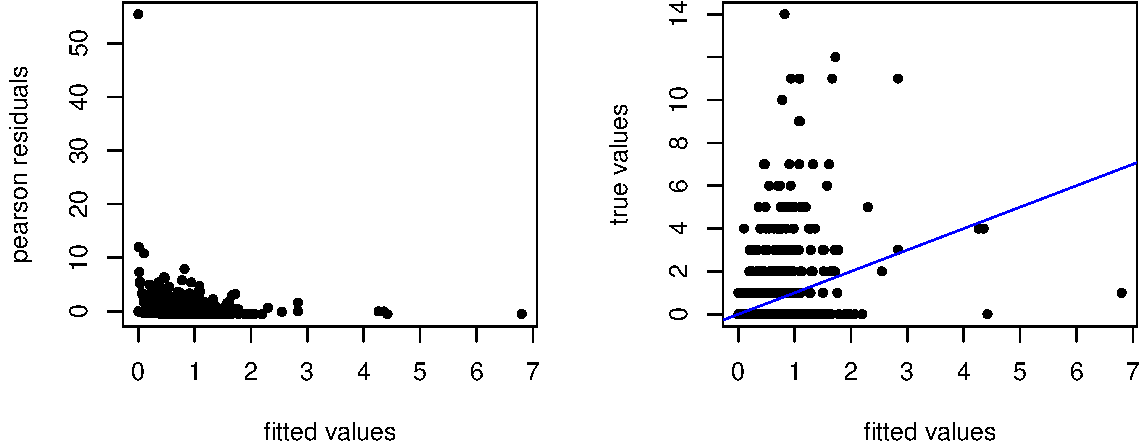
\includegraphics{stats504_hw1_files/figure-latex/unnamed-chunk-5-1.pdf}

\hypertarget{conclusion}{%
\section{Conclusion}\label{conclusion}}

This analysis is aimed to simply explain the association between the
derogatory reports and the applicant's background factors. While it
seems that there may exist other better estimators for this problem, the
zero-inflated negative binomial regression model seems characterize
derogatory reports well and make great progress towards the origional
possion regression model. In conclusion, \texttt{share}, \texttt{owner}
and \texttt{active} are certainly associated to the number of
applicant's derogatory reports.

\hypertarget{appendix}{%
\section{Appendix}\label{appendix}}

\hypertarget{zero-inflated-negative-binomial-regression-model}{%
\subsection{Zero-Inflated Negative Binomial Regression
Model}\label{zero-inflated-negative-binomial-regression-model}}

Suppose that for each observation, there are two possible cases. Suppose
that if case 1 occurs, the count is zero. However if case 2 occurs,
counts(including 0) are generated according to the negative binomial
model. Suppose that case 1 occurs with probability \(\pi\) and case 2
occurs with probability \(1-\pi\). Therefore, the probability
distribution of the ZINB random variable \(y_i\) can be written as

\[
P(y_i = j) = 
\begin{cases}
\pi_i + (1+\pi_i) g(y_i=0) & \text{if }j=0 \\
(1-\pi_i) g(y_i)           & \text{if }j>0
\end{cases}
\] where \(\pi_i\) is the logistic link function defined below and
\(g(y_i)\) is the negative binomial distribution given by \[
g(y_i) = \frac{\Gamma(y_i + 1/\alpha)}{\Gamma(1/\alpha) \Gamma(y_i+1)}\left( \frac{1}{1 + \alpha \mu_i}\right)^{1/\alpha}\left( \frac{\alpha \mu_i}{1 + \alpha \mu_i}\right)^{y_i}.
\] The expression relating these quantities is \[
\mu_i = \exp(\beta_0 + \beta_1 x_1 + \cdots + \beta_k x_k)
\]

The logistic link function \(\pi_i\) is given by \[
\pi_i = \frac{\lambda_i}{1 + \lambda_i}
\] where \[
\lambda_i = \exp(1 + \gamma_0 + \gamma_1 z_1 + \cdots + \gamma_m z_m).
\]

Here \(z\)'s are the variable modeled zero part and \(x\)'s are the
variable modeled for count part.

\hypertarget{code}{%
\subsection{Code}\label{code}}

Source code of this report can be found
\href{https://github.com/ZhihaoXu/Stats504/blob/main/Assignment/assignment_1/stats504_hw1.Rmd}{\emph{here}}.

\begin{Shaded}
\begin{Highlighting}[]
\NormalTok{data =}\StringTok{ }\KeywordTok{read.csv}\NormalTok{(}\StringTok{'derogatory.csv'}\NormalTok{)}
\NormalTok{data =}\StringTok{ }\NormalTok{data }\OperatorTok\StringTok{ }
\StringTok{  }\KeywordTok{select}\NormalTok{(}\OperatorTok{-}\NormalTok{card) }\OperatorTok
\StringTok{  }\KeywordTok{mutate}\NormalTok{(}
    \DataTypeTok{reports =} \KeywordTok{as.integer}\NormalTok{(reports),}
    \DataTypeTok{owner =} \KeywordTok{ifelse}\NormalTok{(data[}\StringTok{'owner'}\NormalTok{]}\OperatorTok{==}\StringTok{'yes'}\NormalTok{, }\DecValTok{1}\NormalTok{, }\DecValTok{0}\NormalTok{),}
    \DataTypeTok{selfemp =} \KeywordTok{ifelse}\NormalTok{(data[}\StringTok{'selfemp'}\NormalTok{]}\OperatorTok{==}\StringTok{'yes'}\NormalTok{, }\DecValTok{1}\NormalTok{, }\DecValTok{0}\NormalTok{),}
    \DataTypeTok{majorcards =} \KeywordTok{ifelse}\NormalTok{(data[}\StringTok{'majorcards'}\NormalTok{]}\OperatorTok{==}\StringTok{'yes'}\NormalTok{, }\DecValTok{1}\NormalTok{, }\DecValTok{0}\NormalTok{)}
\NormalTok{  ) }\OperatorTok
\StringTok{  }\KeywordTok{filter}\NormalTok{(}
\NormalTok{    age }\OperatorTok{>=}\StringTok{ }\DecValTok{18}
\NormalTok{  )}
\end{Highlighting}
\end{Shaded}

\begin{Shaded}
\begin{Highlighting}[]
\NormalTok{expr =}\StringTok{ 'reports ~ age + income + share + expenditure + owner + selfemp + dependents + months + majorcards + active'}
\NormalTok{reportPoission =}\StringTok{ }\KeywordTok{glm}\NormalTok{(expr, }\DataTypeTok{family=}\StringTok{"poisson"}\NormalTok{, }\DataTypeTok{data=}\NormalTok{data)}
\KeywordTok{summary}\NormalTok{(reportPoission)}
\end{Highlighting}
\end{Shaded}

\begin{verbatim}
## 
## Call:
## glm(formula = expr, family = "poisson", data = data)
## 
## Deviance Residuals: 
##     Min       1Q   Median       3Q      Max  
## -3.4424  -0.9615  -0.6672  -0.2576   7.0363  
## 
## Coefficients:
##               Estimate Std. Error z value Pr(>|z|)    
## (Intercept) -6.903e-01  1.889e-01  -3.654 0.000258 ***
## age         -1.237e-03  4.924e-03  -0.251 0.801711    
## income      -3.288e-02  3.080e-02  -1.068 0.285606    
## share       -1.687e+01  2.079e+00  -8.115 4.87e-16 ***
## expenditure  1.303e-03  5.371e-04   2.425 0.015297 *  
## owner       -7.723e-01  1.033e-01  -7.476 7.64e-14 ***
## selfemp     -7.463e-02  1.500e-01  -0.497 0.618902    
## dependents   7.738e-02  3.548e-02   2.181 0.029181 *  
## months       2.573e-03  6.225e-04   4.133 3.58e-05 ***
## majorcards  -2.820e-03  1.058e-01  -0.027 0.978736    
## active       7.686e-02  4.674e-03  16.443  < 2e-16 ***
## ---
## Signif. codes:  0 '***' 0.001 '**' 0.01 '*' 0.05 '.' 0.1 ' ' 1
## 
## (Dispersion parameter for poisson family taken to be 1)
## 
##     Null deviance: 2341.5  on 1311  degrees of freedom
## Residual deviance: 1840.3  on 1301  degrees of freedom
## AIC: 2509.8
## 
## Number of Fisher Scoring iterations: 7
\end{verbatim}

\begin{Shaded}
\begin{Highlighting}[]
\KeywordTok{paste}\NormalTok{(}\StringTok{"AIC of Poisson Regression Model: "}\NormalTok{, }\KeywordTok{AIC}\NormalTok{(reportPoission))}
\end{Highlighting}
\end{Shaded}

\begin{verbatim}
## [1] "AIC of Poisson Regression Model:  2509.80699725031"
\end{verbatim}

\begin{Shaded}
\begin{Highlighting}[]
\KeywordTok{par}\NormalTok{(}\DataTypeTok{mfrow=}\KeywordTok{c}\NormalTok{(}\DecValTok{1}\NormalTok{,}\DecValTok{2}\NormalTok{))}
\KeywordTok{plot}\NormalTok{(reportPoission}\OperatorTok{$}\NormalTok{fitted.values, }\KeywordTok{residuals}\NormalTok{(reportPoission, }\StringTok{'pearson'}\NormalTok{), }
     \DataTypeTok{pch=}\DecValTok{20}\NormalTok{, }\DataTypeTok{xlab=}\StringTok{'fitted values'}\NormalTok{, }\DataTypeTok{ylab=}\StringTok{'pearson residuals'}\NormalTok{)}
\KeywordTok{plot}\NormalTok{(reportPoission}\OperatorTok{$}\NormalTok{fitted.values, data}\OperatorTok{$}\NormalTok{reports,}
     \DataTypeTok{pch=}\DecValTok{20}\NormalTok{, }\DataTypeTok{xlab=}\StringTok{'fitted values'}\NormalTok{, }\DataTypeTok{ylab=}\StringTok{'true values'}\NormalTok{)}
\KeywordTok{abline}\NormalTok{(}\DecValTok{0}\NormalTok{,}\DecValTok{1}\NormalTok{, }\DataTypeTok{col=}\StringTok{'blue'}\NormalTok{)}
\end{Highlighting}
\end{Shaded}

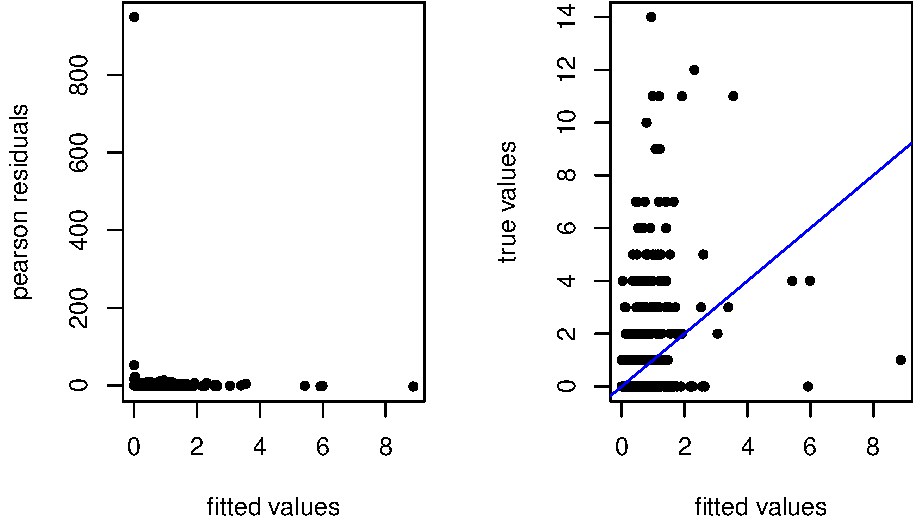
\includegraphics{stats504_hw1_files/figure-latex/unnamed-chunk-8-1.pdf}

\begin{Shaded}
\begin{Highlighting}[]
\NormalTok{reportsZifPos=}\StringTok{ }\KeywordTok{zeroinfl}\NormalTok{(reports }\OperatorTok{~}\StringTok{ }\NormalTok{age }\OperatorTok{+}\StringTok{ }\NormalTok{income }\OperatorTok{+}\StringTok{ }\NormalTok{share }\OperatorTok{+}\StringTok{ }\NormalTok{expenditure }\OperatorTok{+}\StringTok{ }\NormalTok{owner }\OperatorTok{+}\StringTok{ }
\StringTok{                          }\NormalTok{selfemp }\OperatorTok{+}\StringTok{ }\NormalTok{dependents }\OperatorTok{+}\StringTok{ }\NormalTok{months }\OperatorTok{+}\StringTok{ }\NormalTok{majorcards }\OperatorTok{+}\StringTok{ }\NormalTok{active }\OperatorTok{|}\StringTok{ }
\StringTok{                          }\NormalTok{age }\OperatorTok{+}\StringTok{ }\NormalTok{income }\OperatorTok{+}\StringTok{ }\NormalTok{share }\OperatorTok{+}\StringTok{ }\NormalTok{expenditure }\OperatorTok{+}\StringTok{ }\NormalTok{owner }\OperatorTok{+}\StringTok{ }
\StringTok{                          }\NormalTok{selfemp }\OperatorTok{+}\StringTok{ }\NormalTok{dependents }\OperatorTok{+}\StringTok{ }\NormalTok{months }\OperatorTok{+}\StringTok{ }\NormalTok{majorcards }\OperatorTok{+}\StringTok{ }\NormalTok{active, }
\NormalTok{                        data, }\DataTypeTok{dist =} \StringTok{'poisson'}\NormalTok{)}
\KeywordTok{summary}\NormalTok{(reportsZifPos)}
\end{Highlighting}
\end{Shaded}

\begin{verbatim}
## 
## Call:
## zeroinfl(formula = reports ~ age + income + share + expenditure + owner + 
##     selfemp + dependents + months + majorcards + active | age + income + 
##     share + expenditure + owner + selfemp + dependents + months + majorcards + 
##     active, data = data, dist = "poisson")
## 
## Pearson residuals:
##      Min       1Q   Median       3Q      Max 
##  -1.5462  -0.4313  -0.3381  -0.2080 101.9882 
## 
## Count model coefficients (poisson with log link):
##               Estimate Std. Error z value Pr(>|z|)    
## (Intercept)  0.8456129  0.2473595   3.419 0.000630 ***
## age         -0.0098473  0.0068375  -1.440 0.149815    
## income      -0.0270250  0.0361341  -0.748 0.454516    
## share       -7.9485575  2.3443995  -3.390 0.000698 ***
## expenditure -0.0001261  0.0005794  -0.218 0.827762    
## owner       -0.4677738  0.1264886  -3.698 0.000217 ***
## selfemp     -0.0150357  0.1837267  -0.082 0.934776    
## dependents   0.0677376  0.0457520   1.481 0.138730    
## months       0.0002445  0.0007584   0.322 0.747145    
## majorcards   0.1848783  0.1279182   1.445 0.148378    
## active       0.0381014  0.0064354   5.921 3.21e-09 ***
## 
## Zero-inflation model coefficients (binomial with logit link):
##               Estimate Std. Error z value Pr(>|z|)    
## (Intercept)  1.8572840  0.4259126   4.361 1.30e-05 ***
## age         -0.0132538  0.0116619  -1.136  0.25575    
## income      -0.0081052  0.0715212  -0.113  0.90977    
## share        3.7858073  4.0567075   0.933  0.35071    
## expenditure -0.0013420  0.0013976  -0.960  0.33697    
## owner        0.5185053  0.2136959   2.426  0.01525 *  
## selfemp     -0.0356391  0.3290250  -0.108  0.91374    
## dependents  -0.0007766  0.0762039  -0.010  0.99187    
## months      -0.0042294  0.0015560  -2.718  0.00657 ** 
## majorcards   0.2964776  0.2316387   1.280  0.20058    
## active      -0.0837341  0.0140095  -5.977 2.27e-09 ***
## ---
## Signif. codes:  0 '***' 0.001 '**' 0.01 '*' 0.05 '.' 0.1 ' ' 1 
## 
## Number of iterations in BFGS optimization: 35 
## Log-likelihood: -1020 on 22 Df
\end{verbatim}

\begin{Shaded}
\begin{Highlighting}[]
\KeywordTok{paste}\NormalTok{(}\StringTok{"AIC of Zero-Inflated Poisson Regression Model: "}\NormalTok{, }\KeywordTok{AIC}\NormalTok{(reportsZifPos))}
\end{Highlighting}
\end{Shaded}

\begin{verbatim}
## [1] "AIC of Zero-Inflated Poisson Regression Model:  2083.9069970046"
\end{verbatim}

\begin{Shaded}
\begin{Highlighting}[]
\KeywordTok{par}\NormalTok{(}\DataTypeTok{mfrow=}\KeywordTok{c}\NormalTok{(}\DecValTok{1}\NormalTok{,}\DecValTok{2}\NormalTok{))}
\KeywordTok{plot}\NormalTok{(reportsZifPos}\OperatorTok{$}\NormalTok{fitted.values, }\KeywordTok{residuals}\NormalTok{(reportsZifPos, }\StringTok{'pearson'}\NormalTok{), }
     \DataTypeTok{pch=}\DecValTok{20}\NormalTok{, }\DataTypeTok{xlab=}\StringTok{'fitted values'}\NormalTok{, }\DataTypeTok{ylab=}\StringTok{'pearson residuals'}\NormalTok{)}
\KeywordTok{plot}\NormalTok{(reportsZifPos}\OperatorTok{$}\NormalTok{fitted.values, data}\OperatorTok{$}\NormalTok{reports,}
     \DataTypeTok{pch=}\DecValTok{20}\NormalTok{, }\DataTypeTok{xlab=}\StringTok{'fitted values'}\NormalTok{, }\DataTypeTok{ylab=}\StringTok{'true values'}\NormalTok{)}
\KeywordTok{abline}\NormalTok{(}\DecValTok{0}\NormalTok{,}\DecValTok{1}\NormalTok{, }\DataTypeTok{col=}\StringTok{'blue'}\NormalTok{)}
\end{Highlighting}
\end{Shaded}

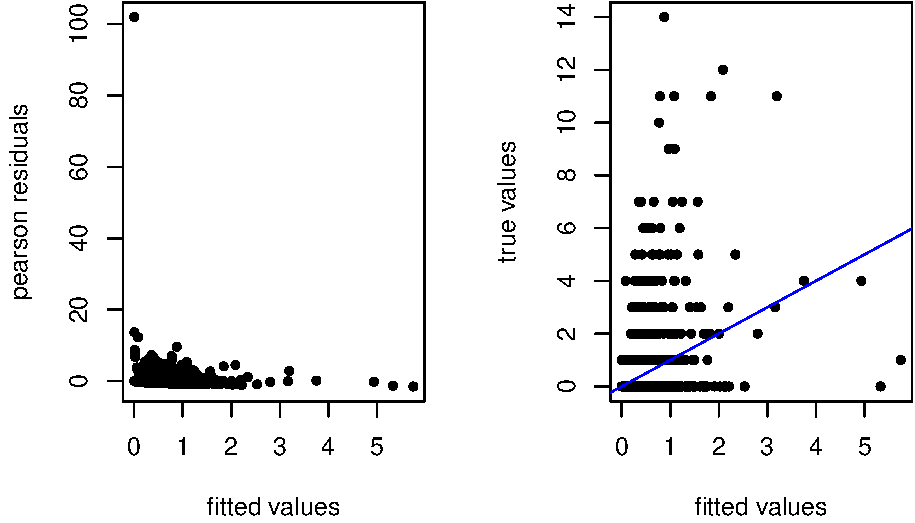
\includegraphics{stats504_hw1_files/figure-latex/unnamed-chunk-10-1.pdf}

\begin{Shaded}
\begin{Highlighting}[]
\NormalTok{reportsZifNB =}\StringTok{ }\KeywordTok{zeroinfl}\NormalTok{(reports }\OperatorTok{~}\StringTok{ }\NormalTok{age }\OperatorTok{+}\StringTok{ }\NormalTok{income }\OperatorTok{+}\StringTok{ }\NormalTok{share }\OperatorTok{+}\StringTok{ }\NormalTok{expenditure }\OperatorTok{+}\StringTok{ }\NormalTok{owner }\OperatorTok{+}\StringTok{ }
\StringTok{                          }\NormalTok{selfemp }\OperatorTok{+}\StringTok{ }\NormalTok{dependents }\OperatorTok{+}\StringTok{ }\NormalTok{months }\OperatorTok{+}\StringTok{ }\NormalTok{majorcards }\OperatorTok{+}\StringTok{ }\NormalTok{active }\OperatorTok{|}\StringTok{ }
\StringTok{                          }\NormalTok{owner }\OperatorTok{+}\StringTok{ }\NormalTok{months }\OperatorTok{+}\StringTok{ }\NormalTok{active, data, }\DataTypeTok{dist =} \StringTok{'negbin'}\NormalTok{)}
\KeywordTok{summary}\NormalTok{(reportsZifNB)}
\end{Highlighting}
\end{Shaded}

\begin{verbatim}
## 
## Call:
## zeroinfl(formula = reports ~ age + income + share + expenditure + owner + 
##     selfemp + dependents + months + majorcards + active | owner + months + 
##     active, data = data, dist = "negbin")
## 
## Pearson residuals:
##        Min         1Q     Median         3Q        Max 
## -5.645e-01 -4.455e-01 -3.439e-01 -4.882e-06  5.546e+01 
## 
## Count model coefficients (negbin with log link):
##               Estimate Std. Error z value Pr(>|z|)    
## (Intercept) -0.9382339  0.3616700  -2.594 0.009482 ** 
## age          0.0051178  0.0091163   0.561 0.574534    
## income       0.0080313  0.0538074   0.149 0.881348    
## share       -8.9709437  2.7189492  -3.299 0.000969 ***
## expenditure  0.0002986  0.0008554   0.349 0.727042    
## owner       -0.8169628  0.1665199  -4.906 9.29e-07 ***
## selfemp     -0.0634994  0.2676749  -0.237 0.812482    
## dependents   0.0796504  0.0625975   1.272 0.203224    
## months       0.0014583  0.0011603   1.257 0.208812    
## majorcards   0.0446625  0.1886809   0.237 0.812882    
## active       0.0666118  0.0131348   5.071 3.95e-07 ***
## Log(theta)  -1.0689430  0.1188873  -8.991  < 2e-16 ***
## 
## Zero-inflation model coefficients (binomial with logit link):
##              Estimate Std. Error z value Pr(>|z|)
## (Intercept)  22.78247  352.32259   0.065    0.948
## owner        -7.14492   85.65965  -0.083    0.934
## months       -0.01109    0.01045  -1.061    0.289
## active      -21.30067  352.30723  -0.060    0.952
## ---
## Signif. codes:  0 '***' 0.001 '**' 0.01 '*' 0.05 '.' 0.1 ' ' 1 
## 
## Theta = 0.3434 
## Number of iterations in BFGS optimization: 67 
## Log-likelihood:  -940 on 16 Df
\end{verbatim}

\begin{Shaded}
\begin{Highlighting}[]
\KeywordTok{paste}\NormalTok{(}\StringTok{"AIC of Zero-Inflated Negative Binomial Regression Model: "}\NormalTok{, }\KeywordTok{AIC}\NormalTok{(reportsZifNB))}
\end{Highlighting}
\end{Shaded}

\begin{verbatim}
## [1] "AIC of Zero-Inflated Negative Binomial Regression Model:  1912.04027211876"
\end{verbatim}

\end{document}
